% Op icon: spline — a smooth curve weaving through marked points.
\documentclass[tikz,border=2mm]{standalone}
\usetikzlibrary{arrows.meta,calc,shapes.geometric}
\begin{document}
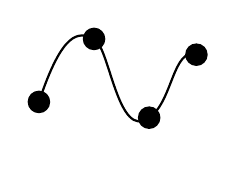
\begin{tikzpicture}[line width=1.3pt, line cap=round, line join=round, >=Stealth, x=1mm,y=1mm]
  \draw[thick]
    (-10,-3) .. controls (-7,6) and (-5,6) .. (-3,5)
             .. controls (-1,4) and (0,-8) .. (4,-5)
             .. controls (7,-3) and (7,4) .. (10,3);
  \foreach \p in {(-10,-3),(-3,5),(4,-5),(10,3)} { \filldraw \p circle (1.2); }
\end{tikzpicture}
\end{document}
